\documentclass{beamer}
\usefonttheme[onlymath]{serif}
\usetheme[numbering=fraction, progressbar=frametitle]{metropolis}
\usepackage{appendixnumberbeamer}
% \setbeamertemplate{navigation symbols}{}
%%% headline section guide
% \useoutertheme[footline=empty,subsection=false]{miniframes}
% \useinnertheme{circles}
%%% if wish no circles on headline
% \setbeamertemplate{headline}{%
%     \begin{beamercolorbox}[colsep=1.5pt]{upper separation line head}
%     \end{beamercolorbox}
%     \begin{beamercolorbox}{section in head/foot}
%     \vskip2pt\insertsectionnavigationhorizontal{\paperwidth}{}{}\vskip2pt
%         \end{beamercolorbox}%
%         \begin{beamercolorbox}[colsep=1.5pt]{lower separation line head}
%     \end{beamercolorbox}
% }

\usepackage{tikz}
\usetikzlibrary{backgrounds}

\usepackage[utf8]{inputenc}
\usepackage[T1]{fontenc}
\usepackage{textcomp}
\usepackage{amsmath, amssymb, amsthm}

\usepackage[style=authoryear,maxbibnames=9,maxcitenames=2,uniquelist=false,backend=biber,doi=false,url=false]{biblatex}
\renewcommand*{\nameyeardelim}{\addcomma\space} % have comma in parencite
\addbibresource{$BIB} % bibtex location
%%% Small bibliography slide
\setbeamertemplate{bibliography item}[triangle]
\makeatletter
\newcommand{\srcsize}{\@setfontsize{\srcsize}{6.5pt}{6.5pt}}
\makeatother
\renewcommand*{\bibfont}{\srcsize}

\usepackage{import}
\usepackage{pdfpages}
\usepackage{transparent}
\usepackage{xcolor}

\newcommand{\blue}[1]{\textcolor{blue}{#1}}
\newcommand{\red}[1]{\textcolor{red}{#1}}

\graphicspath{ {./figures} }
\newcommand{\inkfig}[2][1]{%
    \def\svgwidth{#1\columnwidth}
    \import{./figures/}{#2.pdf_tex}
}

%%%%%% Template
\usepackage{hyperref}
\definecolor{links}{HTML}{2A1B81}

%% beaver (red) style:
% \usecolortheme{beaver}
% \setbeamercolor{block body}{bg=gray!30!white}
% \setbeamercolor{block title}{bg=darkred!70, fg=black!2}
% \hypersetup{colorlinks=true,allcolors=red}

%% seahorse style:
\usecolortheme{seahorse}
\setbeamercolor{block body}{bg=mDarkTeal!30}
\setbeamercolor{block title}{bg=mDarkTeal,fg=black!2}
\hypersetup{colorlinks=true,allcolors=links}
%%%%%% Template

\pdfsuppresswarningpagegroup=1

\title{Unit 14 Supplement}
\author{Hui-Jun Chen}
\institute{The Ohio State University}
\date{\today}

\begin{document}

\maketitle

% \frame{%
%    \maketitle
%    \begin{center}
%        \includegraphics
%			[width=0.2\textwidth]
%			{./figures/Ohio_State_University_seal}
%    \end{center}
% }


\begin{frame}{Multiplier Process}
\label{slide:Multiplier_Process}
    Definition: $ MPC = \frac{\Delta C}{\Delta Y} $

    \begin{columns}
        \begin{column}{0.6\textwidth}
        \begin{itemize}
            \item The initial increase in spending is $ \$x $, from A to B
            \item B will spend $ \$x \times MPC $ back to A
            \item This process continues, and the total increase in GDP is
                    %
                    \begin{equation*}
                        \begin{split}
                                & \$x \cdot 1 + \$x \cdot MPC + \$x \cdot MPC^{2} + \cdots
                            \\
                                & = \$x \cdot ( 1 + MPC + MPC^{2} + \cdots )
                            \\
                                & = \$x \cdot \frac{1}{1 - MPC}
                            \\
                        \end{split}
                    \end{equation*}
                    %
        \end{itemize}
        \end{column}
        \begin{column}{0.5\textwidth}
            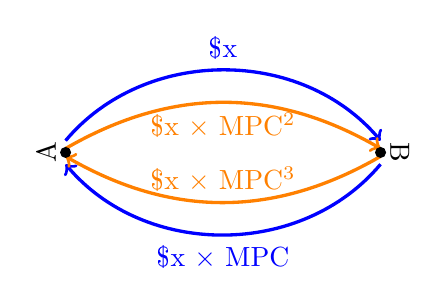
\begin{tikzpicture}
                \pgfmathsetmacro{\x}{5}
                \pgfmathsetmacro{\y}{1}
                % \draw[very thin,color=gray, step=1] (0,0) grid (\x, \y); % gray grid
                \draw[very thick, blue, ->] (1, 0.3) to[bend left=50] node[above]{\$x} (5, 0.3);
                \draw[very thick, blue, <-] (1, 0) to[bend right=50] node[below]{\$x $\times$ MPC} (5, 0);
                \draw[very thick, orange, ->] (1, 0.2) to[bend left=30] node[below]{\$x $\times$ MPC$^2$} (5, 0.2);
                \draw[very thick, orange, <-] (1, 0.1) to[bend right=30] node[above]{\$x $\times$ MPC$^3$} (5, 0.1);
                \fill (1, 0.15) circle (2pt) node[above, rotate=90]{A};
                \fill (5, 0.15) circle (2pt) node[above, rotate=270]{B};
            \end{tikzpicture}
        \end{column}
    \end{columns}




\end{frame}




\metroset{numbering=none}
\printbibliography[heading=none]
% \begin{frame}[allowframebreaks, noframenumbering]
%     \frametitle{References}
%     \printbibliography[heading=none]
% \end{frame}

\end{document}

